% !TEX root = Bachelorarbeit_Paul_Zilewitsch.tex
\section{Umsetzung}

\subsection{Erweiterung des bestehenden Service Desk Moduls}
\noindent
Grundlage für die Erweiterung ist die bereits erwähnte Microsoft Exchange Web Services Managed API 2.2, die kostenlos zum Download von Microsoft angeboten wird. Voraussetzung für diese API ist ein Betriebssystem von Windows (mindestens Windows 7) und das .NET Framwork 3.5 oder höher.\footnote{Website:\cite{DownloadAPI}}\newline 
Da diese API bereits in GEBman10 für das Versenden von E-Mails integriert wurde, konnte direkt ohne zusätzlichen Aufwand auf die Funktionalitäten zugegriffen werden. Wichtig war lediglich das Einfügen des Assemblerverweises in die entsprechenden Projektmappenordner. Um nicht den vollständigen Namespace jeder Klasse ausschreiben zu müssen, wurde außerdem die using-Direktive in den Klassen \textit{MailsToObjectsFactory} und \textit{TicketHandler} hinzugefügt.

\begin{figure}[h!]
\centering
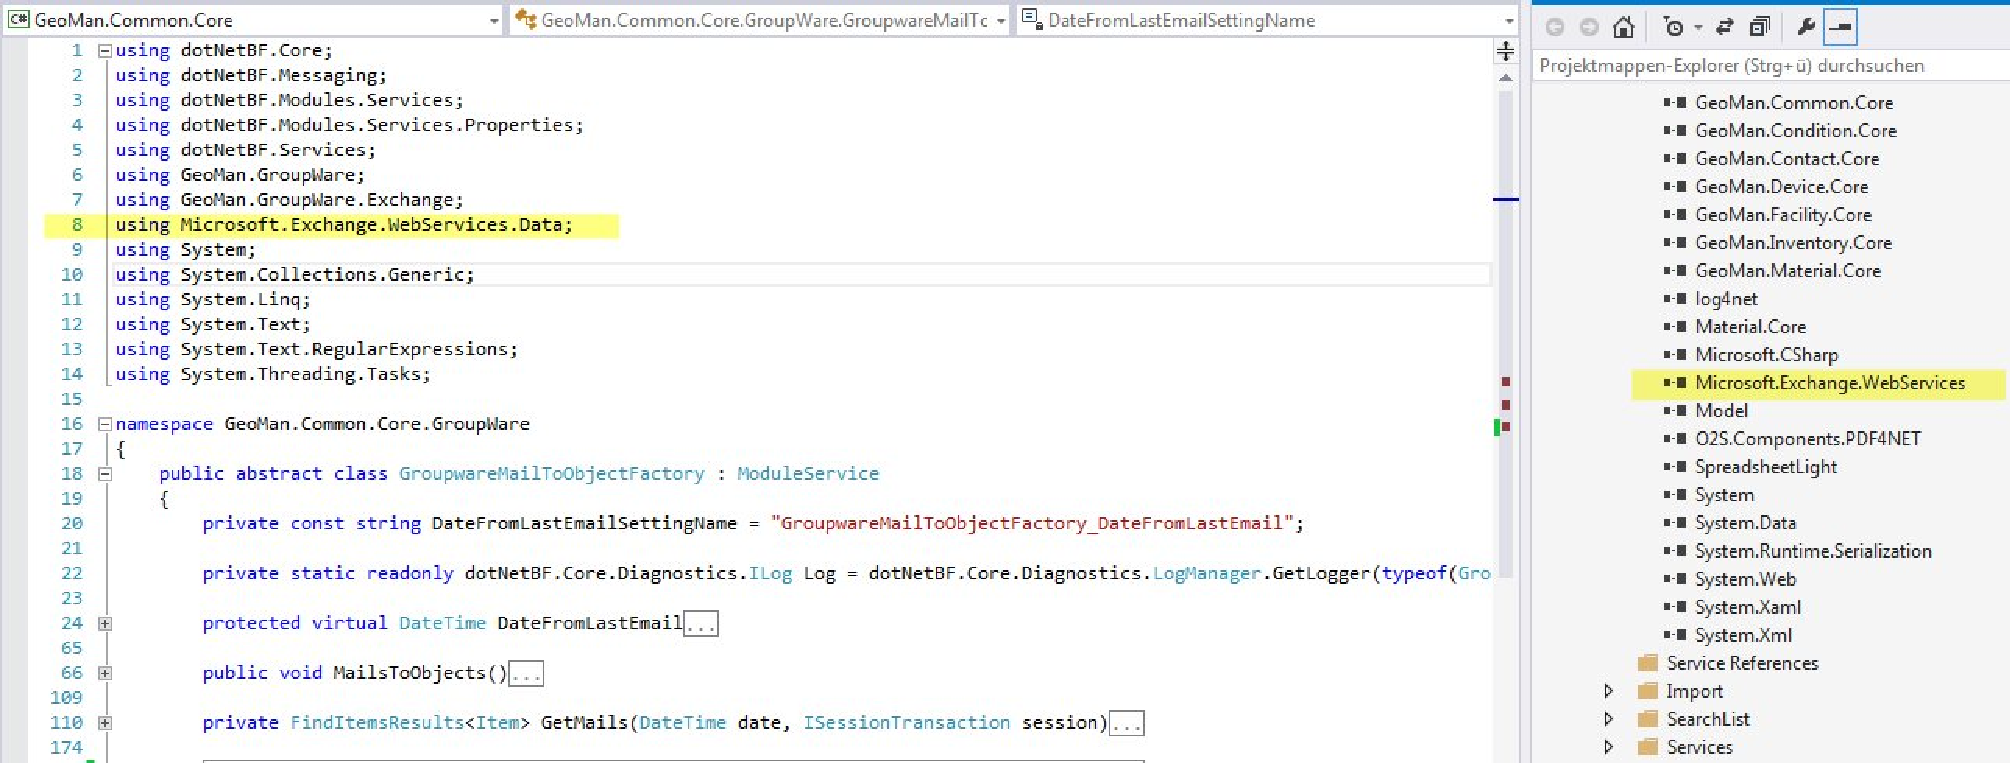
\includegraphics[width=0.75\textwidth]{Abbildungen/Screenshot_Verweise.pdf}
	\caption[Verweise der EWS Managed API]{Verweise der EWS Managed API, Quelle: eigene Darstellung}
	\label{fig:Verweise}
\end{figure}

\noindent
Bei der Implementierung wurde sich stark an das Fabrikmethoden-Entwurfsmuster gehalten. Bevor hierauf näher eingegangen wird, sollte das Entwurfsmuster näher erläutert werden.\\
\noindent
Die Fabrikmethode (Factory Method) ist ein Erzeugungsmuster, bei dem die Objekterstellung von der Objektverarbeitung getrennt wird. Hierbei wird die Unterklasse durch eine abstrakte Methode der Oberklasse erzeugt.\footnote{Vgl. \citeauthor{PatternsKompakt} \citeyear{PatternsKompakt}, S.34ff.} Dieses Entwurfsmuster wurde auch bei der Implementierung in GEBman10 verwendet.\\ 

\begin{figure}[htb]
    \centering
    \begin{minipage}[t]{0.47\textwidth}
        \centering
        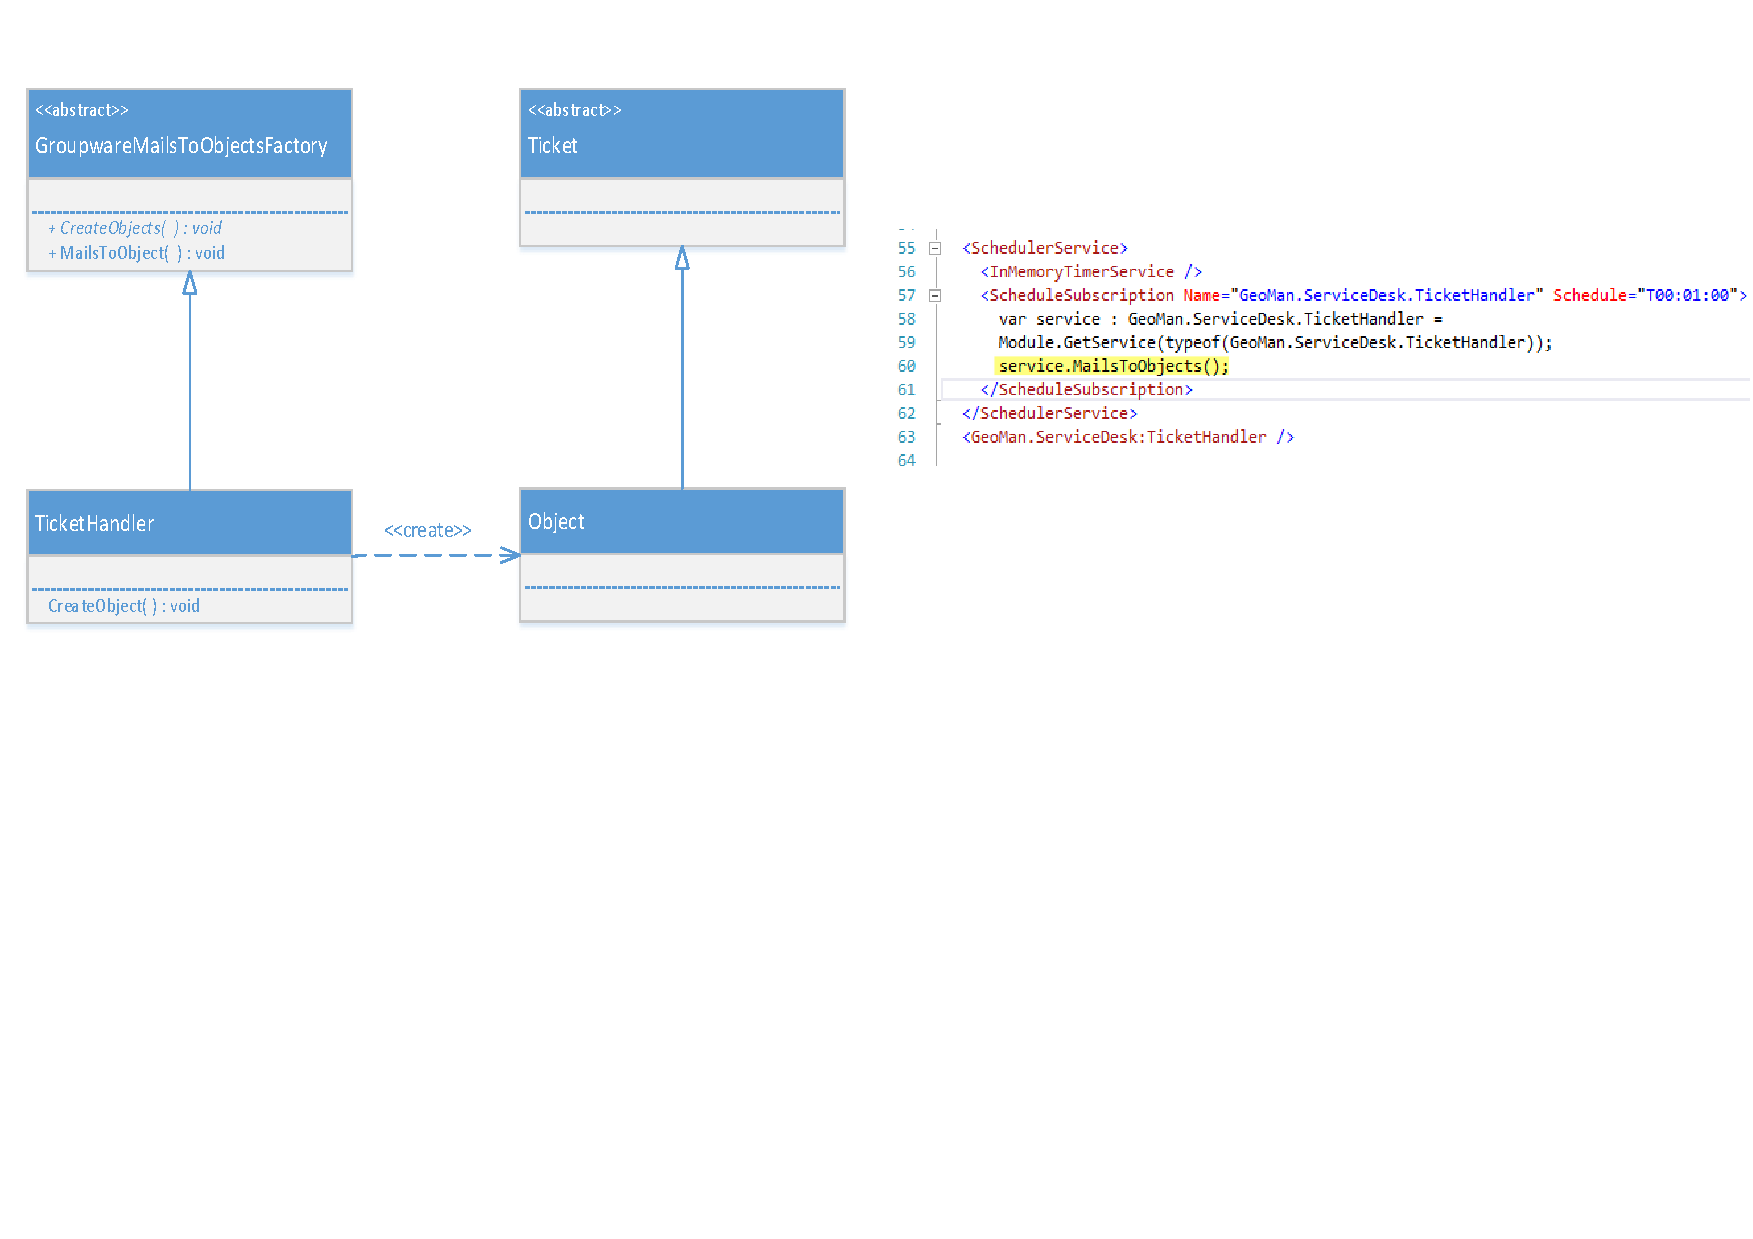
\includegraphics[width=.90\textwidth]{Abbildungen/Entwurfsmuster.pdf}
        \caption[Entwurfsmuster Fabrikmethode]{Entwurfsmuster Fabrikmethode, Quelle: in Anlehnung an Eilebrecht, Starke (2013) S.35}
        \label{fig:Entwurfsmuster}
    \end{minipage}% <- sonst wird hier ein Leerzeichen eingefügt
    \hfill
    \begin{minipage}[t]{0.47\textwidth}
        \centering
        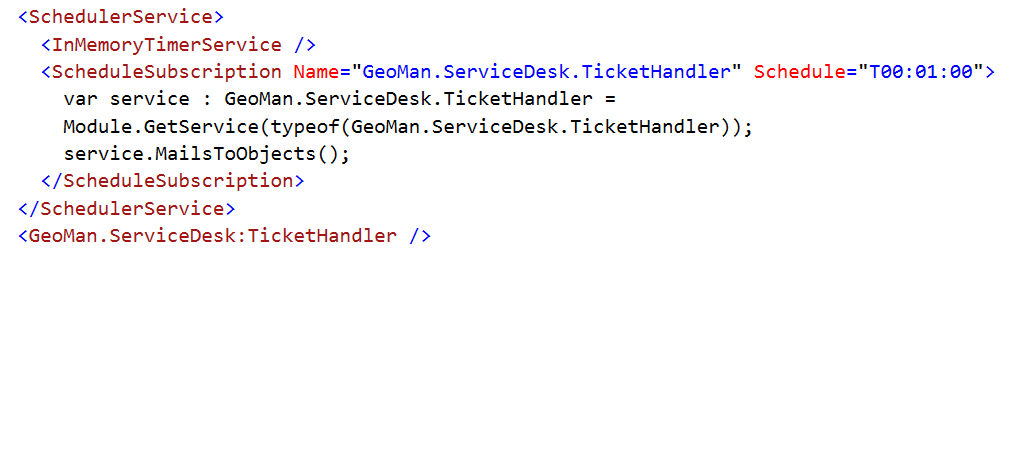
\includegraphics[width=.99\textwidth]{Abbildungen/ModuleService.png}
        \caption[Module Service Aufruf]{Module Service Aufruf, Quelle: eigene Darstellung}
        \label{fig:ModuleService}
    \end{minipage}
\end{figure}

\noindent
Die Fabrikmethode (Abbildung~\ref{fig:Entwurfsmuster}) macht deutlich, dass die abstrakte Klasse \textit{GroupwareMailToObjectFactory} der Erzeuger und \textit{TicketHandler} der konkrete Erzeuger ist. Der konkrete Erzeuger wiederum erstellt dann ein Objekt über die abstrakte Methode \textit{CreateObject( )}. Das Objekt ist in diesem Falle ein Ticket (Meldung). Vorteil dieses Entwurfsmusters ist die klare Kapselung des Erzeugers. Somit kann die Klasse \textit{GroupwareMailToObjectFactory} auch für andere Module eingesetzt werden, die ebenfalls neue Objekte aus E-Mails erzeugen sollen.\\

\noindent
Die beiden Experten für Entwurfsmuster Eilebrecht und Starke sehen die Anwendung der Fabrikmethode als sinnvoll, wenn \enquote{eine Klasse die von ihr zu erzeugenden Objekte nicht im Voraus kennt}.\footnote{\citeauthor{PatternsKompakt} \citeyear{PatternsKompakt}, S.34ff.} Genau dieser Anwendungsfall trifft hier zu und ist deshalb auch gerechtfertigt.\\

\noindent
Bei jedem Intervall wird über den \textit{SchedulerService} (Abbildung~\ref{fig:ModuleService}) der Module Service \textit{TicketHandler} instanziiert und die Methode \textit{MailsToObjects( )} der abstrakten Oberklasse aufgerufen. Das Intervall wurde hier mit \enquote{T00:01:00} bestimmt, was einen Zeitabstand von einer Minute entspricht.




\subsection{Erläuterung einzelner Methoden}
\noindent
Die Methode \textit{GetMails( )} in der Klasse \textit{GroupwareMailsToObjectFactory} ist die entscheidende Methode der Erweiterung bei dem Abrufen der E-Mails eines Exchange Servers. Hier werden nicht nur alle Mails abgerufen, sondern auch verschiedene Attribute der einer E-Mails geladen. Im Anhang auf Seite \pageref{Codeausschnitt} befindet sich ein Codeausschnitt, in dem diese Schritte in der Programmiersprache C\#/.NET implementiert sind. Zu sehen ist hier, wie zunächst alle Exchange Server aus Datenbank in eine Liste gespeichert werden. Darauffolgend wird der erste Server aus der Liste dazu genutzt, einen Exchange Service zu erzeugen. Für den Exchange Service sind Benutzername, Passwort, die Domain und eine Autodiscover URL notwendig, um auf alle Funktionalitäten zugreifen zu können. Nun können auch auch schon alle E-Mails aus dem Postfach des Exchange Servers abgefragt werden. Jedoch müssen einige Eigenschaften (Properties) der E-Mails (Items) erst geladen werden, bevor auf sie verwendet werden können. Alle für den weiteren Verlauf benötigten Eigenschaften sind in der Variablen  \textit{additionalProperties} definiert und werden mit der Methode  \textit{LoadPropertiesForItems( )} geladen. Der Exchange Service speichert alle E-Mails (Items), die er gefunden hat, in die  \textit{ItemCollection result}, die am Ende der Methode  \textit{GetMails( )} den Rückgabewert bildet. 

\noindent
Das erstellen einer Meldung (bzw. eines Objektes) erfolgt in der Methode \textit{CreateObject( )}. Diese Methode ist in der \textit{GroupwareMailsToObjectFatory} als abstrakte Methode definiert, wird der Klasse \textit{TicketHandler} vererbt und hier auch explizit aufgerufen. Wichtig bei diese Methode ist die Übergabe einer Session. In GEBman10 benötigt jede Datenbankbearbeitung eine neue \textit{SessionTransaction}.\footnote{Vgl. \citeauthor{Fowler} \citeyear{Fowler}, S.103ff.} 
Mithilfe der Session lässt sich somit auf die Create-Methode der Ticket Klasse zugreifen. Anschließend werden die Eigenschaften des E-Mail-Items den zuvor angedeuteten nötigen Eigenschaften eines Tickets zugewiesen. Nach diesem Prozess wird die Session \textit{committed}, um die neu erstellte Meldung in der Datenbank zu speichern. Erst jetzt erhält die Meldung eine eindeutige ID. Diese ID kann dazu genutzt werden, um im nächsten Schritt einen möglichen Anhang der E-Mail zu speichern. Das übernimmt die Methode \textit{SaveAttachment( )}. In dieser Methode wird zunächst ein Dokument mit dem selben Inhalt des Anhangs der E-Mail erstellt. Dann wird dieses Dokument dem entsprechenden Ticket mit Hilfe der übergebenen ID zugeordnet. Wurden diese Anweisungen erfolgreich durchgeführt, wird eine Bestätigungsmail mit der Methode \textit{SendConfirmationMail( )} gesendet.\\

\noindent
Bei jedem Versuch die Datenbank zu verändern, kann es zu Fehlern kommen, die dem Benutzer auch mitgeteilt werden müssen. Der Benutzer muss schließlich darüber informiert werden, wenn eine Meldung nicht korrekt angelegt wurde. Aus diesem Grund wurden try-catch-Anweisungen bei jedem Datenbankzugriff verwendet. Durch diese try-catch-Anweisungen werden Ausnahmen beim Ausführen des Codes abgefangen. Dadurch ist es möglich, eine Ausnahmebehandlung zu vollziehen.\footnote{Website:\cite{TryCatch}}\\


\subsection{Testfälle}
\noindent
In den letzten Jahren hat sich das Testen von Software zunehmende etabliert und ist ein fester Bestandteil von Softwareprojekten für die Qualitätssicherung.\footnote{Vgl.\citeauthor{Vivenzio} \citeyear{Vivenzio}, S.1f.} Deshalb werden auch bei der Erweiterung des Service Desk Moduls einige Testfälle die wichtigsten Funktionalitäten überprüfen. Hierfür muss zunächst ein Testablauf erarbeitet und ein die zu erwartenden Werte des Testresultats festgehalten werden.\newline
Bei den Testfällen in GEBman 10 wird im ersten Schritt der Webserver gestartet. Dadurch wird auch der implementierte Modul Service \textit{TicketHandler} initialisiert. Nun werden alle Modultests ausgeführt. Für den Test des Module Service wird ein Exchange Server benötigt. Dieser wird mittels einer Methode in der \textit{TestHelper}-Klasse angelegt. An diesen Exchange Service wird eine E-Mail gesendet und anschließend der Module Service aufgerufen. Theoretisch könnte der Modultest auch bis zum nächsten Intervall des Modul Service warten, bis dieser die neuesten Mails vom Exchange Server abfragt. Doch ein Modultest sollte so wenig Zeit wie möglich beanspruchen. Aus diesem Grund wird die Methode \textit{MailsToObjects ( )} vom Module Service manuell aufgerufen. Eine neue Meldung wird aus der zuvor gesendeten E-Mail erstellt. Erst jetzt beginnt der eigentliche Test. Es wird eine Datenbankabfrage erstellt, die nach der Meldung sucht, die der Module Service angelegt haben müsste. Sollte die Abfrage erfolglos sein, wird der Modultest mit einem Fehler beendet. Sollte die Meldung gefunden werden, wird im nächsten Schritt geprüft, ob der Anhang der E-Mail als Dokument der Meldung angelegt wurde. Wurde kein Dokument gefunden, dass der zuvor erstellten Meldung zugeordnet ist, schlägt der Modultest fehl und eine entsprechende Meldung wird ausgegeben.\newline
Die Testfälle können noch weiter ausgebaut werden, in dem weitere Methoden implementiert werden, die eine erfolgreiche Antworterstellung oder das Versenden von Bestätigungsmails prüfen. Abschließend ist festzuhalten, dass niemals alle möglichen Szenarien in Testfällen berücksichtigt werden können, aber auch gar nicht müssen. Es geht lediglich darum, die Szenarien zu testen, die am häufigsten in der Praxis auftreten.\footnote{Vgl.\citeauthor{Witte} \citeyear{Witte}, S.11f.}\\


\subsection{Fehlschläge/Erfahrungen}
\noindent
Bei der Implementierung in GEBman10 gab es zwei nicht vorhersehbare Probleme bei der Implementierung. Beide haben ihren Ursprung in der Managed API von Microsoft. In der Methode \textit{GetMails( )} werden alle Mails aus dem Posteingang des Exchange Servers abgefragt. Hierfür stellt die API eine Methode namens \textit{FindItems( )} zur Verfügung, die eine \textit{Collection} aller Items liefert. Nun muss aber für diese Collection eine ItemView übergeben werden, die einen bestimmten Integerzahlenwert als festdefinierte Größe benötigt. Es ist also in der Theorie durchaus möglich, dass sich mehr Mails im Posteingang des Exchange Server befinden, als die Menge an Elementen der \textit{ItemView}. Das hat zur Folge, dass alle Mails außerhalb der \textit{ItemView} nicht in die \textit{Collection} von der Methode \textit{FindItems( )} enthalten sind und auch nicht ausgewertet werden können. Um dieses Problem kurzer Hand zu beseitigen, wurde die ItemView Größe auf den maximalen Zahlenwert des Integerwertebereiches gesetzt. Dieses Wert zu überschreiten ist in der Praxis so gut wie unmöglich, der sich in einem 10-stelligen Bereich bewegt.\\
%Es gäbe noch einen anderen WorkAround für dieses Problem, allerdings wäre diese Lösung mit mehr Aufwand verbunden. 
%https://msdn.microsoft.com/en-us/library/office/dd633698(v=exchg.80).aspx

\noindent
Das zweite Problem bestand bei der Abfrage der neusten Mails vom Exchange Server, ebenfalls in der \textit{GetMails( )}-Methode beschrieben. Bei jedem Abfrage Intervall wird der Zeitpunkt der zuletzt eingetroffenen Mail gespeichert. Beim nächsten Intervalldurchlauf werden dann nur alle Mails abgefragt, die ein aktuelles Datum besitzen. Hierfür bietet die Managed API einen \textit{SearchFilter} an, der die Mails nach definierten Eigenschaften suchen kann. In diesem Fall ist war die Filter-Methode \textit{IsGreatherThan( )} optimal für dieses Vorhaben. Theoretisch hätten alle Mails abgefragt werden müssen, die ein \enquote{größeres} und damit aktuelleres Datum als die zuletzt eingetroffene Mail vom vorherigen Intervalldurchlauf hatten. Tatsächlich hat sich beim Debuggen gezeigt, dass der Filter zusätzlich ebenfalls die Mails liefert, die das gleiche Datum besitzen. Dadurch würde eine Mail in jedem Intervall zweimal gefiltert werden, was eine womöglich redundante Objekterzeugung zur Folge hätte. Wodurch dieses Problem entstand bleibt unklar. Umgangen wurde es, indem dem Datum der zuletzt eingetroffenen Mail nur eine Sekunde hinzugefügt wurde. Nach dieser minimalen Veränderung wurden die Mails korrekt gefiltert.


\subsection{Erweiterungsmöglichkeiten der E-Mail Integration}
\noindent
Die E-Mail Integration könnte dahingehend erweitert werden, dass der Benutzer mit einer E-Mail mehr Möglichkeiten zum Verändern vorhandener Meldungen hat. Sollte ein Benutzer beispielsweise den Status einer Meldung auf \enquote{Technisch fertig setzen} setzen wollen, könnt er das über eine E-Mail bewerkstelligen, ohne dabei in GEBman 10 eingeloggt sein zu müssen. Denkbar wäre es, in den Betreff der E-Mail einen Parameter wie \enquote{\#fertig} einzusetzen. Beim Auslesen der E-Mails durch den Module Service könnte das erkannt werden und dem Absender der E-Mail könnte ein Link geschickt werden. Mit diesem Link könnte der Benutzer dann zu einem temporären Webfrontend gelangen, auf dem dann die Fertigstellung der Meldung noch einmal bestätigt.\\

\noindent
In GEBman 10 können mehrere Benutzer mit ihren E-Mail Adressen hinterlegt werden. Der Modul Service könnte abgleichen, ob ein Absender einer E-Mail im Exchange Postfach eine identische E-Mail Adresse wie ein registrierter Benutzer in GEBman 10 hat. Ist die E-Mail Adressen eines hinterlegten Benutzer identisch mit der E-Mail Adresse eines Absenders für eine neue Meldung, kann in der Meldung im Service Desk-Modul direkt der registrierte Benutzer als Melder eingetragen werden. Die Eigenschaft Melder ist zwar nicht unbedingt notwendig, dadurch kann eine Meldung aber besser gefiltert werden und man hat direkte Einsicht darauf, an wen man sich bei Fragen wenden kann.\\

\noindent
Des Weiteren wird in der prototypischen Implementierung die Abfrage der E-Mails nur für ein Exchange Server aus der Datenbank durchgeführt. Es ist in GEBman 10 aber durchaus möglich, mehrere Exchange Server zu konfigurieren. Diese zusätzlichen Server werden derzeit noch nicht berücksichtigt und demzufolge werden auch keine E-Mails abgerufen. Da alle Exchange Server im Programmcode in eine Liste gespeichert werden, sollte dies jedoch keine große Hürde darstellen.

